\documentclass[t]{beamer}

\subtitle{What Is Number Theory}

\usepackage{amsthm,amsmath,amsfonts,hyperref,graphicx,color,multicol,soul}
\usepackage{enumitem,tikz,tikz-cd,setspace,mathtools}

%%%%%%%%%%
%Beamer Template Customization
%%%%%%%%%%
\setbeamertemplate{navigation symbols}{}
\setbeamertemplate{theorems}[ams style]
\setbeamertemplate{blocks}[rounded]

\definecolor{Blu}{RGB}{43,62,133} % UWEC Blue
\setbeamercolor{structure}{fg=Blu} % Titles

%Unnumbered footnotes:
\newcommand{\blfootnote}[1]{%
	\begingroup
	\renewcommand\thefootnote{}\footnote{#1}%
	\addtocounter{footnote}{-1}%
	\endgroup
}

%%%%%%%%%%
%TikZ Stuff
%%%%%%%%%%
\usetikzlibrary{arrows}
\usetikzlibrary{shapes.geometric}
\tikzset{
	smaller/.style={
		draw,
		regular polygon,
		regular polygon sides=3,
		fill=white,
		node distance=2cm,
		minimum height=1in,
		line width = 2pt
	}
}
\tikzset{
	smsquare/.style={
		draw,
		regular polygon,
		regular polygon sides=4,
		fill=white,
		node distance=2cm,
		minimum height=1in,
		line width = 2pt
	}
}


%%%%%%%%%%
%Custom Commands
%%%%%%%%%%

\newcommand{\C}{\mathbb{C}}
\newcommand{\quats}{\mathbb{H}}
\newcommand{\N}{\mathbb{N}}
\newcommand{\Q}{\mathbb{Q}}
\newcommand{\R}{\mathbb{R}}
\newcommand{\Z}{\mathbb{Z}}

\newcommand{\ds}{\displaystyle}

\newcommand{\fn}{\insertframenumber}

\newcommand{\id}{\operatorname{id}}
\newcommand{\im}{\operatorname{im}}
\newcommand{\lcm}{\operatorname{lcm}}
\newcommand{\Aut}{\operatorname{Aut}}
\newcommand{\Inn}{\operatorname{Inn}}

\newcommand{\blank}[1]{\underline{\hspace*{#1}}}

\newcommand{\abar}{\overline{a}}
\newcommand{\bbar}{\overline{b}}
\newcommand{\cbar}{\overline{c}}

\newcommand{\nml}{\unlhd}

%%%%%%%%%%
%Custom Theorem Environments
%%%%%%%%%%
\theoremstyle{definition}
\newtheorem{exercise}{Exercise}
\newtheorem{question}[exercise]{Question}
\newtheorem{warmup}{Warm-Up}
\newtheorem*{exa}{Example}
\newtheorem*{disc}{Group Discussion}
\newtheorem*{recall}{Recall}
\renewcommand{\emph}[1]{{\color{blue}\texttt{#1}}}

\definecolor{Gold}{RGB}{237, 172, 26}
%Statement block
\newenvironment{statementblock}[1]{%
	\setbeamercolor{block body}{bg=Gold!20}
	\setbeamercolor{block title}{bg=Gold}
	\begin{block}{\textbf{#1.}}}{\end{block}}
\newenvironment{goldblock}{%
	\setbeamercolor{block body}{bg=Gold!20}
	\setbeamercolor{block title}{bg=Gold}
	\setbeamertemplate{blocks}[shadow=true]
	\begin{block}{}}{\end{block}}
\newenvironment{defn}{%
	\setbeamercolor{block body}{bg=gray!20}
	\setbeamercolor{block title}{bg=violet, fg=white}
	\setbeamertemplate{blocks}[shadow=true]
	\begin{block}{\textbf{Definition.}}}{\end{block}}
\newenvironment{nb}{%
	\setbeamercolor{block body}{bg=gray!20}
	\setbeamercolor{block title}{bg=teal, fg=white}
	\setbeamertemplate{blocks}[shadow=true]
	\begin{block}{\textbf{Note.}}}{\end{block}}
\newenvironment{blockexample}{%
	\setbeamercolor{block body}{bg=gray!20}
	\setbeamercolor{block title}{bg=Blu, fg=white}
	\setbeamertemplate{blocks}[shadow=true]
	\begin{block}{\textbf{Example.}}}{\end{block}}
\newenvironment{blocknonexample}{%
	\setbeamercolor{block body}{bg=gray!20}
	\setbeamercolor{block title}{bg=purple, fg=white}
	\setbeamertemplate{blocks}[shadow=true]
	\begin{block}{\textbf{Non-Example.}}}{\end{block}}
\newenvironment{thm}[1]{%
	\setbeamercolor{block body}{bg=Gold!20}
	\setbeamercolor{block title}{bg=Gold}
	\begin{block}{\textbf{Theorem #1.}}}{\end{block}}


%%%%%%%%%%
%Custom Environment Wrappers
%%%%%%%%%%
\newcommand{\exer}[1]{
	\begin{exercise}
		#1
	\end{exercise}
}
\newcommand{\exam}[1]{
\begin{blockexample}
	#1
\end{blockexample}
}
\newcommand{\nexam}[1]{
\begin{blocknonexample}
	#1
\end{blocknonexample}
}
\newcommand{\enumarabic}[1]{
	\begin{enumerate}[label=\textbf{\arabic*.}]
		#1
	\end{enumerate}
}
\newcommand{\enumalph}[1]{
	\begin{enumerate}[label=(\alph*)]
		#1
	\end{enumerate}
}
\newcommand{\bulletize}[1]{
	\begin{itemize}[label=$\bullet$]
		#1
	\end{itemize}
}
\newcommand{\circtize}[1]{
	\begin{itemize}[label=$\circ$]
		#1
	\end{itemize}
}
\newcommand{\slide}[1]{
	\begin{frame}{\fn}
		#1
	\end{frame}
}
\newcommand{\slidec}[1]{
\begin{frame}[c]{\fn}
	#1
\end{frame}
}
\newcommand{\slidet}[2]{
	\begin{frame}{\fn\ - #1}
		#2
	\end{frame}
}


\newcommand{\startdoc}{
		\title{Math 341: Classical Number Theory}
		\author{Mckenzie West}
		\date{Last Updated: \today}
		\begin{frame}
			\maketitle
		\end{frame}
}

\newcommand{\topics}[2]{
	\begin{frame}[c]{\insertframenumber}
		\begin{block}{\textbf{Last Section.}}
			\begin{itemize}[label=--]
				#1
			\end{itemize}
		\end{block}
		\begin{block}{\textbf{This Section.}}
			\begin{itemize}[label=--]
				#2
			\end{itemize}
		\end{block}
	\end{frame}
}

\begin{document} 
	\startdoc
	
	\topics{
		% Last Time
		\item Hmmm....
	}
	{
		% This time
		\item Introduction to Number Theory 
			
			We will spend 2-3 days on these slides and on this topic.
	}

\slidec{
	\begin{question}
		What is Number Theory and what is its purpose?
	\end{question}
	\begin{defn}
		\emph{Pure mathematics} is the study of mathematical concepts independently of any application outside mathematics.
		
		\emph{Number Theory} is a branch of pure mathematics devoted primarily to the study of the integers.
	\end{defn}
}

\slidec{
	\begin{goldblock}
		``[Number theory] produces, without effort, innumerable problems which have a sweet, innocent air about them, tempting flowers; and yet…number theory swarms with bugs, waiting to bite the tempted flower-lovers who, once bitten, are inspired to excesses of effort!''
	
	(Barry Mazur, "Number Theory as Gadfly", The American Mathematical Monthly, Volume 98, 1991)
	\end{goldblock}
}

\slidec{
	\begin{question}
		Why study Number Theory?
		\bulletize{
			\item The beauty and elegance of the statements of the claims.
			\item The beauty and elegance of the proofs of the claims.
			\item The pleasure one receives from understanding the proofs.
			\item Beauty.
		}
	\end{question}
}
\slidec{
	\begin{goldblock}
		``Thank God that
		number theory is unsullied by any application.''
		
		(Leonard Dickson 1874--1954, Year Unknown)
	\end{goldblock}
\vskip .25in
	\begin{goldblock}
		``...virtually every theorem in elementary number theory arises in a natural, motivated
		way in connection with the problem of making computers do high-speed
		numerical calculations.''
		
		(Donald Knuth, 1974)
	\end{goldblock}
}

\slide{
	\begin{block}{\textbf{Srinivasa Ramanujan.}}
		\begin{minipage}{.7\textwidth}
			\bulletize{
				\item Indian Mathematician
				\item Lived 1887-1920
				\item Had little formal training in mathematics
				\item Produced almost 3,900 results, mostly identities and equations.
				\item Began correspondence with G.H.~Hardy in 1913.
			}
		\end{minipage}
		\begin{minipage}{.25\textwidth}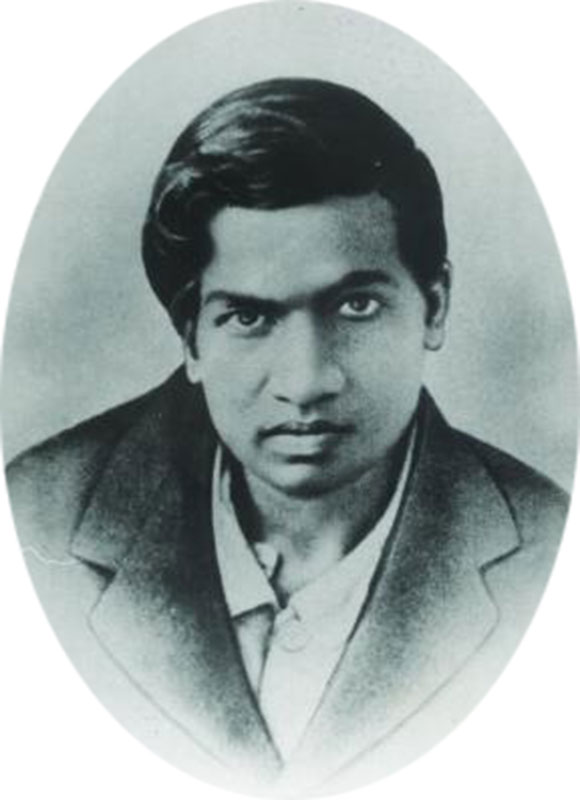
\includegraphics[width=\textwidth]{ramanujan}\end{minipage}
	\end{block}
	\begin{goldblock}
		``An equation for me has no meaning unless
		it expresses a thought of God.''
		
		(Srinivasa Ramanujan)
	\end{goldblock}
	\begin{goldblock}
	``They must be true, because if they were not true, no one would have had the imagination to invent them.''
	
	(G.H.~Hardy)
	\end{goldblock}
}

\slide{
\begin{statementblock}{Ramanujan's Series for $\pi$}
	\[\pi=\frac{9801}{2\sqrt 2}\left(\sum_{k=0}^\infty \frac{(4k)!\cdot(1103+26390k)}{(k!)^4\cdot396^{4k}}\right)^{-1}\]
\end{statementblock}
\exer{
	\enumalph{
		\item How good is the estimate if we just truncate to the first term of the sum.
		\item How about 2 terms?
	}
}
\begin{nb}
	This sum converges exponentially (FAST) and is used for some of the fastest algorithms for computing $\pi$.
\end{nb}
}

\slide{
	\begin{statementblock}{Ramanujan's Tantalizing Continued Fraction}
		In a letter to Hardy in 1913, Ramanujan wrote:
		\[\cfrac{1}{1+
			\cfrac{e^{-2\pi}}{1+
				\cfrac{e^{-4\pi}}{1+
					\cfrac{e^{-6\pi}}{1+
						\cfrac{e^{-8\pi}}{1+
							\ddots}}}}}=\left(\sqrt{\frac{5+\sqrt 5}{2}}-\frac{1+\sqrt{5}}{2}\right)\sqrt[5]{e^{2\pi}}\]
	\end{statementblock}
}

\slide{
	\begin{statementblock}{Ramanujan's Tantalizing Nested Radical}
		\[3=\sqrt{1+2\sqrt{1+3\sqrt{1+4\sqrt{1+5\sqrt{1+\cdots}}}}}.\]
	\end{statementblock}
	\vskip 3in\mbox{}
}

\slide{
	\begin{statementblock}{Theorem 0.6 (Ramanujan's Second Notebook, Chapter XII, entry 4)}
		The following identity holds,
		\[x+n+a=\sqrt{ax+(n+a)^2+x\sqrt{a(x+n)+(n+a)^2+(x+n)\sqrt{\cdots}}}\]
	\end{statementblock}
	Read more: \url{https://www.sciencedirect.com/science/article/pii/S0377042704001906}
	\begin{question}
		What do we get if we take $x=2$, $n=1$ and $a=0$?
	\end{question}
}

\slidet{Typical Number Theory Questions}{
	\begin{question}
		Can a sum of two squares be a square?
	\end{question}
	\vskip 1in
	\begin{question}
		Can a sum of two cubes be a cube?
	\end{question}
	\vskip 1in\mbox{}
}

\slidet{Typical Number Theory Questions}{
	\begin{question}
		Regarding prime numbers (positive integers $p>1$ such that its only divisors are 1 and $p$ itself):
		\enumarabic{
			\item Are there infinitely many primes?
			\item Are there infinitely many primes of the form $4k+1$ where $k$ is an integer?
			\item Are there infinitely many primes of the form $4k+3$ where $k$ is an integer?
		}
	\end{question}
	\vskip 2in\mbox{}
}
\slidet{Typical Number Theory Questions}{
\begin{question}
	Are there infinitely many twin primes? That is, are there
	infinitely many primes p such that p + 2 is also prime?
\end{question}
Here are the first several twin prime pairs:
$$(3, 5), (5, 7), (11, 13), (17, 19), (29, 31), (41, 43), (59, 61),$$
$$(71, 73), (101, 103), (107, 109), (137, 139), \dots$$
\vskip 1in\mbox{}
}
\slidet{Typical Number Theory Questions}{
\begin{question}
	What, if anything, is significant about the even integer
	lying between each pair, excluding the first pair $(3,5)$?
\end{question}
Here are the first several twin prime pairs again.
$$(3, 5), (5, 7), (11, 13), (17, 19), (29, 31), (41, 43), (59, 61),$$
$$(71, 73), (101, 103), (107, 109), (137, 139), \dots$$
\vskip 1in\mbox{}
}
\slidet{Typical Number Theory Questions}{
\begin{question}
	Is $\sqrt 2$ irrational?
\end{question}
\vskip 1in
\begin{question}
	If $i=\sqrt{-1}$ is $i^i$ a real number?
\end{question}
\vskip 1in\mbox{}
}
\slidet{Typical Number Theory Questions}{
\begin{question}
	Are there infinitely many primes of the form $n^2+1$?
\end{question}
Here are some values:
$$\begin{array}{|l||l|c|}
	\hline
	\mathbf{n}&\mathbf{n^2+1}&\text{\textbf{Is Prime?}}\\
	\hline\hline
	2&2^2+1=5&\text{ True }\\\hline
	4&4^2+1=17&\text{ True }\\\hline
	6&6^2+1=37&\text{ True }\\\hline
	8&8^2+1=65&\text{ False }\\\hline
	10&10^2+1=101&\text{ True }\\\hline
	12&12^2+1=145&\text{ False }\\\hline
	14&14^2+1=197&\text{ True }\\\hline
	16&16^2+1=257&\text{ True }\\\hline
	18&18^2+1=325&\text{ False }\\\hline
	20&20^2+1=401&\text{ True }\\\hline
	22&22^2+1=485&\text{ False }\\\hline
	24&24^2+1=577&\text{ True }\\\hline
\end{array}$$
\vskip 1in\mbox{}
}
\slide{
\begin{statementblock}{Four Famous Conjectures}
	\begin{description}\setlength{\itemsep}{2em}
		\item[Goldbach's Conjecture] Can every even integer greater than 2 be written as the sum of two primes?
		\item[Twin Prime Conjecture] Are there infinitely many primes $p$ such that $p+2$ is also prime?
		\item[Legendre's Conjecture] Does there always exist at least one prime between consecutive perfect squares?
		\item[Landau's Conjecture] Are there infinitely many primes $p$ such that $p-1$ is a perfect square.
	\end{description}
\end{statementblock}
}
\slide{
	\begin{question}
		Which positive integers are the sum of two squares?
	\end{question}

	Here are all of them that are less than 100:
	\begin{center}
		\begin{tabular}{ccccccccccc}
		1&2&4&5&8&9&10&13&16&17&18\\
		20&25&26&29&32&34&36&37&40&41&45\\
		49&50&52&53&58&61&64&65&68&72&73\\
		74&80&81&82&85&89&90&97&98
		\end{tabular}
	\end{center}
	\begin{exercise}
		What is special about the primes that appear in this list?
	\end{exercise}\vskip .5in
	\begin{exercise}
		What is special about the primes factors of the numbers that appear in this list?
	\end{exercise}
	\vskip 1in \mbox{}
}

\slide{
	\begin{statementblock}{Erd\v os--Straus Conjectures}
		For all integers $n\geq 2$, the rational number $\frac{4}{n}$ can be expressed as the sum of three positive unit fractions (fractions of the form $\frac{1}{k}$).  For example, when $n=5$,
			\[\frac{4}{5}=\frac{1}{2}+\frac{1}{5}+\frac{1}{10}.\]
	\end{statementblock}

	\begin{nb}
		Computer searches have confirmed this for $n\leq 10^{17}$.
	\end{nb}
}

%\slide{
%\begin{statementblock}{Brocard's Problem}
%	What integers $n,m$ satisfy $n!+1=m^2$? 
%\end{statementblock}
%\begin{exercise}
%	Verify that $n=4,5,7$ satisfy such an equation.\vskip 3in\mbox{}
%\end{exercise}
%}
%\slide{
%\begin{statementblock}{Conjecture (Brocard, 1876 and 1855) and (Ramanujan, 1913)}
%	 $n=4,5,7$ are the only values that makes this work.
%\end{statementblock}
%}
\slide{
	\begin{statementblock}{Brocard's Conjecture}
		There are at least four prime numbers between $(p_n)^2$ and $(p_{n+1})^2$, for $n\geq 2$, where $p_n$ is the $n$th prime number.
	\end{statementblock}
	\begin{exercise}
		Verify this statement for $n=2,3$.\vskip 3in\mbox{}
	\end{exercise}
}
\slide{
	\begin{statementblock}{Reimann Hypothesis}
		Define the Riemann-zeta function to be the infinite series
			\[\zeta(s)=\sum_{n=1}^\infty n^{-s}=\frac{1}{1^s}+\frac{1}{2^s}+\frac{1}{3^s}+\frac{1}{4^s}+\cdots.\]
		This series \textit{converges absolutely} if $s$ is a complex number with real part greater than 1. 
		
		Using the method of ``analytic continuation'' $\zeta(s)$ can be defined for all complex numbers aside from $s=1$.
		
		\textbf{Conjecture.} $\zeta(s)=0$ exactly when $s$ is a negative even integer or $s=\frac{1}{2}+ri$ for some $r\in\R$.
	\end{statementblock}
}
\slide{
	\begin{center}
		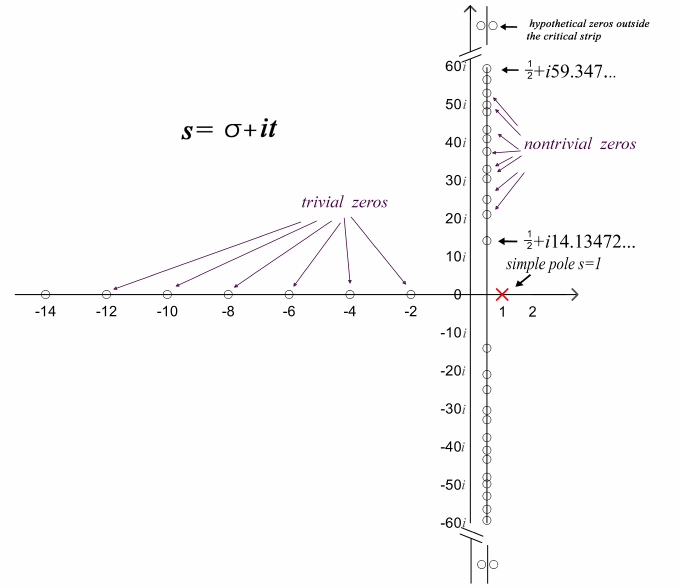
\includegraphics[width=.75\textwidth]{riemann_hypothesis}
	\end{center}
}
\slidet{Some Good News!}{
		\begin{statementblock}{Conjecture (Fermat, c.~1637) Theorem (Wiles, 1995)}
			The equation $a^n+b^n=c^n$ has no non-trivial integer solutions $(a,b,c)$ if $n\geq 3$.
		\end{statementblock}
		\begin{proof}[Proof Idea]
			\enumalph{
				\item \textbf{Fact:} The general equation for FLT is elliptic.
				\item \textbf{Taniyama--Shimura--Weil (TSW) Conjecture, 1967:} Each rational elliptic curve is also a modular form.
				\item \textbf{Frey's Conjecture, 1986:} Any counterexample to FLT would also imply that a semistable elliptic curve existed that was not modular.
				\item \textbf{Ribet, 1990:} Frey's conjecture holds.
				\item \textbf{Wiles, 1995:} Wiles proves TSW's conjecture holds.
			}
		\end{proof}
}
\slide{
	\begin{exa}
		If there are 10 pigeons and only 9 holes, then if all 10 pigeons are to fly into holes, then at least one hole will contain more than on pigeon.
		\begin{center}
			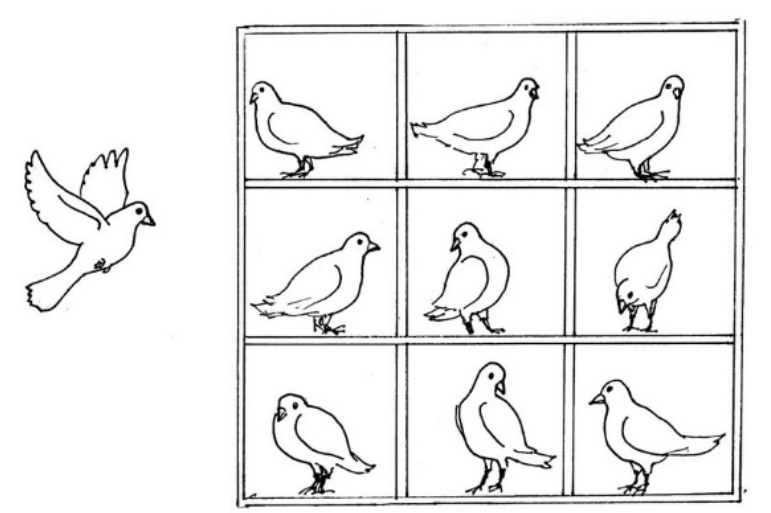
\includegraphics[width=3in]{php}
		\end{center}
	\end{exa}
}
\slide{
	\begin{statementblock}{Pigeonhole Principle}
		If $m$ and $n$ are positive integers with $m<n$, then if we are to place $n$ objects in $m$ containers then at least one container will contain more than one object.
	\end{statementblock}\vskip 2in\mbox{}
}
\slide{
	\begin{statementblock}{Lemma}
		If $a,b\in\Z$ and leave the same remainder when divided by some $d\in\Z$, then $d$ divides $a-b$.
	\end{statementblock}	
	\begin{exercise}
		Verify this for $a=51$, $b=16$, and $d=7$.
		\begin{eqnarray*}
			51&=&\fbox{\color{white}ASDF}\cdot7+\fbox{\color{white}ASDF},\\
			16&=&\fbox{\color{white}ASDF}\cdot7+\fbox{\color{white}ASDF}.
		\end{eqnarray*}
		Thus we see
		\[51-16=(\fbox{\color{white}ASDF}-\fbox{\color{white}ASDF})\cdot 7.\]
	\end{exercise}
}
%\slide{
%	\begin{statementblock}{Lemma}
%		If $a,b\in\Z$ and leave the same remainder when divided by some $d\in\Z$, then $d$ divides $a-b$.
%	\end{statementblock}	
%	\begin{proof}
%		Let $a,b,d\in\Z$.  Assume $a$ and $b$ have the same remainder when divided by $d$.\vskip 3in
%	\end{proof}
%}
\slide{
	\begin{statementblock}{A fun result}
		Consider the following sequence of integers with repeating digits:
		\[1,11,111,1111,11111,111111,\dots\]
		There is at least one term in this sequence divisible by 2023.
	\end{statementblock}
	\begin{proof}
		We will prove that one of the first 2023 terms is divisible by 2023.  For notation, assume that $y_i$ is the $i$th term in the sequence and let $(y_i)_{i=1}^{2023}$ denote the sequence of the first 2023 terms.
		
		Assume toward contradiction that for every $1\leq i\leq 2023$, none of the $y_i$ is divisible by 2023.  Set $r_i$ to be the remainder when dividing $y_i$ by 2023.  \vskip 1in
	\end{proof}
}
\slide{
	\begin{proof}[Continuing]
		Observe the following
		\bulletize{
			\item $0<r_i<2023$ for all $i$ \fbox{WHY}\vskip .5in
			\item there are at least two equal $r$ values	\fbox{WHY}\vskip .5in
		}
		We denote two equal remainders $r_j$ and $r_k$ for some $r,k$ with $1\leq j<k\leq 2023$. Consider $y_k-y_j$.\vskip 2in
	\end{proof}
}
\slide{
	\begin{proof}[Continuing]
		Observe the following
		\bulletize{
			\item $y_k-y_j$ leaves a remainder of 0 upon dividing by 2023 \fbox{WHY}\vskip .25in
			\item $y_k-y_j$ equals $y_{k-j}\cdot 10^j$.	\fbox{WHY}\vskip .5in
			\item 2023 divides $y_{k-j}\cdot 10^j$, and thus divides $y_{k-j}$.	\fbox{WHY}\vskip .5in
		}
		Therefore, we have a contradiction.	\fbox{WHY}\vskip .25in
		We conclude that some term in the sequence $(y_i)_{i=1}^{2023}$ is divisible by 2023.
	\end{proof}
}
\slide{
	\begin{statementblock}{Afterthoughts and Remarks/Questions}
		\bulletize{
			\item Was there anything special about the ones?  For example, does 2023 divide some term in the sequence
			\[2, 22, 222, 2222, 22222, 222222,\dots?\]\vskip .5in
			\item Was there anything special about 2023? For example, can we replace the 2023 with 2022 and use the same proof.\vskip .5in
			\item This is called an \emph{existence proof} because it does not tell us which term is divisible by 2023 only that \textit{some} term is divisible by 2023.
		}
	\end{statementblock}
}
\slide{
	\begin{exercise}
		For you to think about.
		$$\begin{array}{|c||l|c|}
			\hline
			n&y_n&21|y_n\\\hline\hline
			1&1&False\\\hline
			2&11&False\\\hline
			3&111&False\\\hline
			4&1111&False\\\hline
			5&11111&False\\\hline
			6&111111&True\\\hline
			7&1111111&False\\\hline
			8&11111111&False\\\hline
			9&111111111&False\\\hline
		\end{array}\hskip 2em
		\begin{array}{|c||l|c|}
			\hline
			n&y_n&21|y_n\\\hline\hline
			10&1111111111&False\\\hline
			11&11111111111&False\\\hline
			12&111111111111&True\\\hline
			13&1111111111111&False\\\hline
			14&11111111111111&False\\\hline
			15&111111111111111&False\\\hline
			16&1111111111111111&False\\\hline
			17&11111111111111111&False\\\hline
			18&111111111111111111&True\\\hline
		\end{array}$$
		
		Make a conjecture about the values $y_n$ divisible by 21.
	\end{exercise}
}
\slide{
	\begin{statementblock}{Theorem}
		The sum $1+2+3+\cdots+n$ equals $\ds\frac{n(n+1)}{2}$.
	\end{statementblock}
	\begin{block}{\textbf{Picture.}}
		\begin{center}
			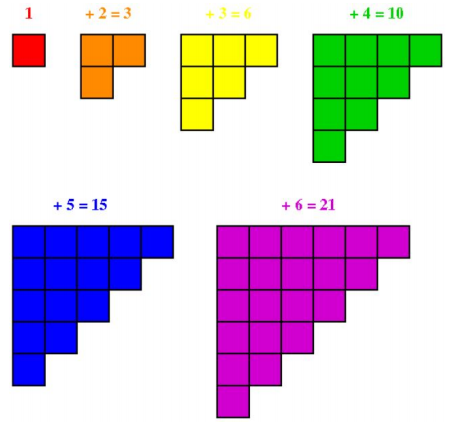
\includegraphics[width=2in]{integer_sum}
		\end{center}
	\end{block}
}
\slide{
	\begin{statementblock}{Theorem}
		The sum $1^3+2^3+3^3+\cdots+n^3$ equals $\ds\frac{n^4+2n^3+n^2}{4}$.
	\end{statementblock}
	\begin{exercise}
		Let's look past the ``ugliness'' and see if we actually believe this statement.
		$$\begin{array}{|c||c|c|c|}
			\hline
			n&1^3+2^3+\cdots+n^3&\frac{n^4+2n^3+n^2}{4}&\text{Equal}?\\\hline\hline
			1&&&\\\hline
			2&&&\\\hline
			3&&&\\\hline
			4&&&\\\hline
			5&&&\\\hline
		\end{array}$$
	\end{exercise}
}
\slide{
	\begin{exercise}
		Re-write the last theorem by simplifying $\frac{n^4+2n^3+n^2}{4}$.\vskip 3in\mbox{}
	\end{exercise}
}
\slide{
	\begin{statementblock}{Theorem}
		\[1^3+2^3+3^3+\cdots +n^3 = (1+2+3+\cdots+n)^2\]
	\end{statementblock}
	\begin{exercise}
		How do these pictures ``prove'' the re-written version?
		\begin{center}
			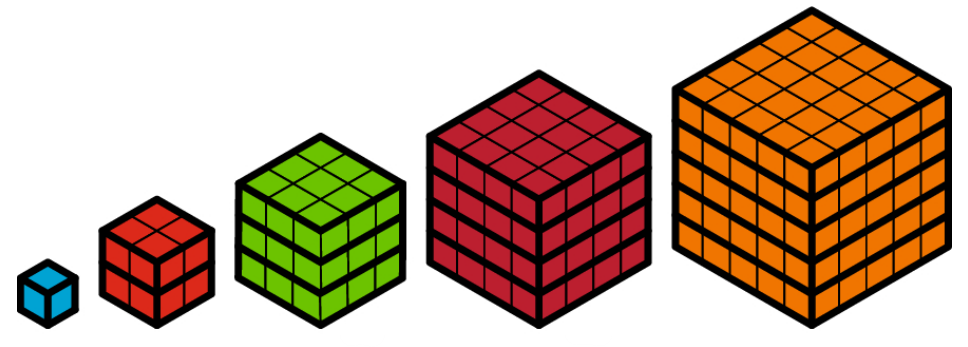
\includegraphics[width=2in]{unit_cubes}\hskip2em
			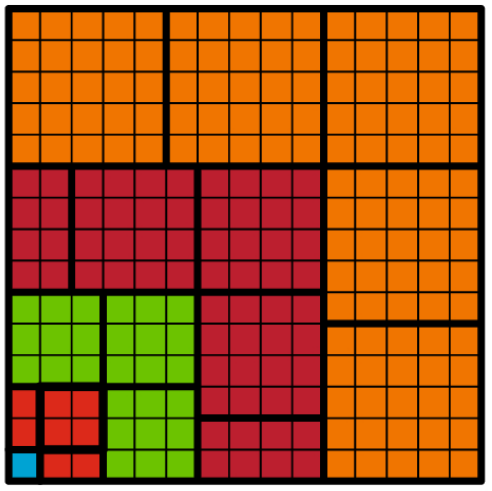
\includegraphics[width=1.5in]{cube_friends}
		\end{center}
	\end{exercise}
}
\end{document}

